\begin{qBox}{3}
Determine \( T_{ C } \) from the specific heat per spin, \( C / N \).
Do this for lattice sizes of \( 20 \times 20 \), \( 50 \times 50 \), 
\( 100 \times 100 \), and combine the results in a single plot.
Comment on how the \( T_{ C } \) values you obtain compare.

\tcblower

Below shows the plot that I was able to produce: 

\begin{figure}[H]
    \centering
    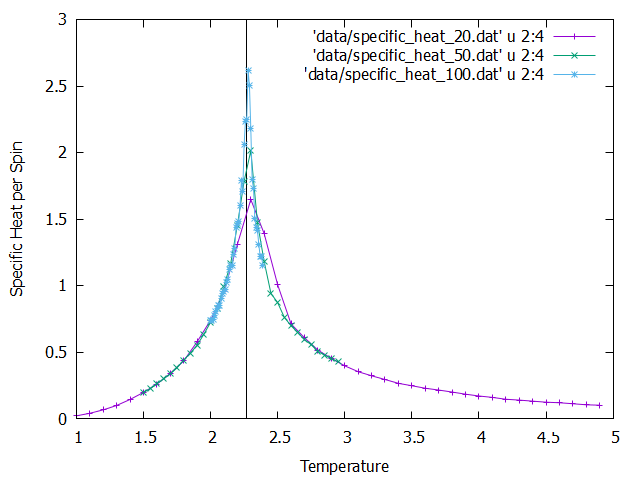
\includegraphics[ width = 0.5\linewidth ]{figures/assignment6_3.png}
    \caption{My plot for \( C / N \) vs \( T \) with a vertical line around %
    \( T_{ C } \)}
\end{figure}

From the plot above, we can see that 
\begin{equation*}
    20 \times 20: 
    T_{ C } \approx 2.30
    \qquad 
    50 \times 50: 
    T_{ C } \approx 2.29
    \qquad 
    100 \times 100: 
    T_{ C } \approx 2.27
\end{equation*}
Notice that as the lattice size increases, we have the peak to both be closer to 
\( T_{ C } \) as well as larger and sharper.
We expect this to be the case since the peak in \( C / N \) becomes 
sharper as lattice size increases -- in fact, \( C_{ \text{max} } / N \sim \log ( L ) \)
as noted in lecture.
If we were to continue with larger lattice sizes, then we should expect the peak 
to be almost asymptotic. 
\end{qBox}